\section{Introduction}

\plt{The introduction section is written to introduce the problem.  It starts
  general and focuses on the problem domain. The general advice is to start with
a paragraph or two that describes the problem, followed by a ``roadmap''
paragraph.  A roadmap orients the reader by telling them what sub-sections to
expect in the Introduction section.}

Do you know the game Yahtzee? Played with dice, it's like Poker but more varied, requiring different skills, without betting. It uses 5 dice, with the usual dots representing the numbers 1 to 6. In rolling the dice, players try to create specific formations, thereby scoring points. At the end of a set number of rounds of dice rolls, the player with the higher score wins.
But the cube isn't the only possibility for dice as the octahedron, with 8 sides could be used. Scoring could likewise be done each round. The number of dice could be changed. These suggest an expanded version of Yahtzee.
This project creates an online multiplayer game platform that allows for the creation of custom Yahtzee-like games and variants. This family of games will come with some presets such as classic Yahtzee, Dr. Paul's octahedron version, and more, but will allow for the users to set their own variables such as number of dice, what kind of dice, and some elements of scoring, and then play that game. Kinds of dice would include cubes and octahedrons, among other multi-sided dice, and scoring could be calculated at the end of the game, as in classic Yahtzee, or on a per-round basis, where hands go in a head-to-head matchup.

This section includes a general overview of the entire SRS document providing descriptions of all sections. It also outlines of the areas of knowledge needed to grasp the documentation accurately.

\subsection{Purpose of Document}

\plt{This section summarizes the purpose of the SRS document.  It does not focus
  on the problem itself.  The problem is described in the ``Problem
  Description'' section (Section~\ref{Sec_pd}).  The purpose is for the document
  in the context of the project itself, not in the context of this course.
  Although the ``purpose'' of the document is to get a grade, you should not
  mention this.  Instead, ``fake it'' as if this is a real project.  The purpose
  section will be similar between projects.  The purpose of the document is the
  purpose of the SRS, including communication, planning for the design stage,
  etc.}

  The Software Requirements Specification (SRS) document aims to clearly define the functional and non-functional needs of the project in order so that all parties involved have a common understanding of the objectives and requirements of the project. Throughout the whole software lifecycle, the SRS will serve as the development team's fundamental guide, aiding in the phases of design, implementation, and testing. ⁤⁤In addition, it facilitates effective communication between stakeholders and creates a framework that ensures the end result satisfies user requirements and is in line with the project's pre-determined goals.
  
  \subsection{Scope of Requirements} 

\plt{Modelling the real world requires simplification.  The full complexity of
  the actual physics, chemistry, biology is too much for existing models, and
  for existing computational solution techniques.  Rather than say what is in
  the scope, it is usually easier to say what is not.  You can think of it as
  the scope is initially everything, and then it is constrained to create the
  actual scope.  For instance, the problem can be restricted to 2 dimensions, or
  it can ignore the effect of temperature (or pressure) on the material
  properties, etc.}  

\plt{The scope section is related to the assumptions section
  (Section~\ref{sec_assumpt}).  However, the scope and the assumptions are not
  at the same level of abstraction.  The scope is at a high level.  The focus is
  on the ``big picture'' assumptions.  The assumptions section lists, and
  describes, all of the assumptions.}

\plt{The scope section is relevant for later determining typical values of inputs. The scope should make it clear what inputs are reasonable to expect. This is a distinction between scope and context (context is a later section).  Scope affects the inputs while context affects how the software will be used.}

The scope of the project involves developing a modified Yahtzee game that features adjustable numbers of playable dice and various game attribute variations. This game will be available for both offline and online play, offering single-player and multiplayer. The scope does not include the implementation of advanced graphics, advanced computer opponents and other board games.

\subsection{Characteristics of Intended Reader} \label{sec_IntendedReader}

\plt{This section summarizes the skills and knowledge of the readers of the
  SRS.  It does NOT have the same purpose as the ``User Characteristics''
  section (Section~\ref{SecUserCharacteristics}).  The intended readers are the
  people that will read, review and maintain the SRS.  They are the people that
  will conceivably design the software that is intended to meet the
  requirements.  The user, on the other hand, is the person that uses the
  software that is built.  They may never read this SRS document.  Of course,
  the same person could be a ``user'' and an ``intended reader.''}

\plt{The intended reader characteristics should be written as unambiguously and
  as specifically as possible.  Rather than say, the user should have an
  understanding of physics, say what kind of physics and at what level.  For
  instance, is high school physics adequate, or should the reader have had a
  graduate course on advanced quantum mechanics?}

  The intended readers of this SRS document are mainly software developers and game designers with expertise in 3D game development and design using game engines, in this case Godot. They should possess a solid understanding of game mechanics, particularly those related to dice games, and have experience with 3D modelling and physics simulations. Additionally, experience with C# and .NET is necessary for readers due to the development being done using C# on a.NET framework. A university-level undergraduate understanding of probability theory is also crucial for comprehending the game's underlying mechanics and probabilities due to the differing number of playable dice. It is assumed that readers are well-versed in these areas.

\subsection{Organization of Document}

\plt{This section provides a roadmap of the SRS document.  It will help the
  reader orient themselves.  It will provide direction that will help them
  select which sections they want to read, and in what order.  This section will
  be similar between project.}

This SRS document is structured to provide a clear roadmap for readers. The sections are as follows:

\begin{itemize}
    \item \textbf{Introduction} 
    \begin{itemize}
        \item Outlines the purpose and scope of the SRS.
    \end{itemize}
    
    \item \textbf{General System Description} 
    \begin{itemize}
        \item Outlines an overview of the project, along with user characterstics, system constraint and the interfaces between the system and its environment.
    \end{itemize}
    
    \item \textbf{Specific System Description} 
    \begin{itemize}
        \item Indepth system description containg  high-level probelem and goal description, along with solutions characteristics, assumptions, definiations and instance models  detailed functionalities and features of the system.
    \end{itemize}
    
    \item \textbf{Requirements} 
    \begin{itemize}
        \item Outlines both functional and non-functional requirements of the system.
    \end{itemize}
    
    \item \textbf{Likely Changes} 
    \begin{itemize}
        \item Outlines anticipated modifications to the system.
    \end{itemize}
    
    \item \textbf{Unlikely Changes} 
    \begin{itemize}
        \item Outlines ascpects of the system that will remain static.
    \end{itemize}
    
    \item \textbf{Traceability Matrices and Graphs} 
    \begin{itemize}
        \item Tracking of requirements throughout the development process.
    \end{itemize}
    
    \item \textbf{Development Plan} 
    \begin{itemize}
        \item Outlines the general timeline and milestones for the project.
    \end{itemize}
    
    \item \textbf{Values of Auxiliary Constants} 
    \begin{itemize}
        \item Outlines constant parameters used in report.
    \end{itemize}
    
    \item \textbf{Commonalities} 
    \begin{itemize}
        \item Outlines commonalities between differnt aspects of the system.
    \end{itemize}
    
    \item \textbf{Variabilities} 
    \begin{itemize}
        \item Outlines variables between differnt aspects of the system.
    \end{itemize}
    
    \item \textbf{Parameters of Variations} 
    \begin{itemize}
        \item Outlines the different variations of aspects of the system.
    \end{itemize}
    
    \item \textbf{Appendix — Reflection} 
    \begin{itemize}
        \item Indepth insights into the development process and lessons learned.
    \end{itemize}
\end{itemize}


\newpage
\section{General System Description}

This section provides general information about the system.  It identifies the
interfaces between the system and its environment, describes the user
characteristics and lists the system constraints.  \plt{This text can likely be
  borrowed verbatim.}

\plt{The purpose of this section is to provide general information about the
  system so the specific requirements in the next section will be easier to
  understand. The general system description section is designed to be
  changeable independent of changes to the functional requirements documented in
  the specific system description. The general system description provides a
  context for a family of related models.  The general description can stay the
  same, while specific details are changed between family members.}

\subsection{System Context}

\plt{Your system context will include a figure that shows the abstract view of
  the software.  Often in a scientific context, the program can be viewed
  abstractly following the design pattern of Inputs $\rightarrow$ Calculations
  $\rightarrow$ Outputs.  The system context will therefore often follow this
  pattern.  The user provides inputs, the system does the calculations, and then
  provides the outputs to the user.  The figure should not show all of the
  inputs, just an abstract view of the main categories of inputs (like material
  properties, geometry, etc.).  Likewise, the outputs should be presented from
  an abstract point of view.  In some cases the diagram will show other external
  entities, besides the user.  For instance, when the software product is a
  library, the user will be another software program, not an actual end user.
  If there are system constraints that the software must work with external
  libraries, these libraries can also be shown on the System Context diagram.
  They should only be named with a specific library name if this is required by
  the system constraint.}

\begin{figure}[h!]
\begin{center}
 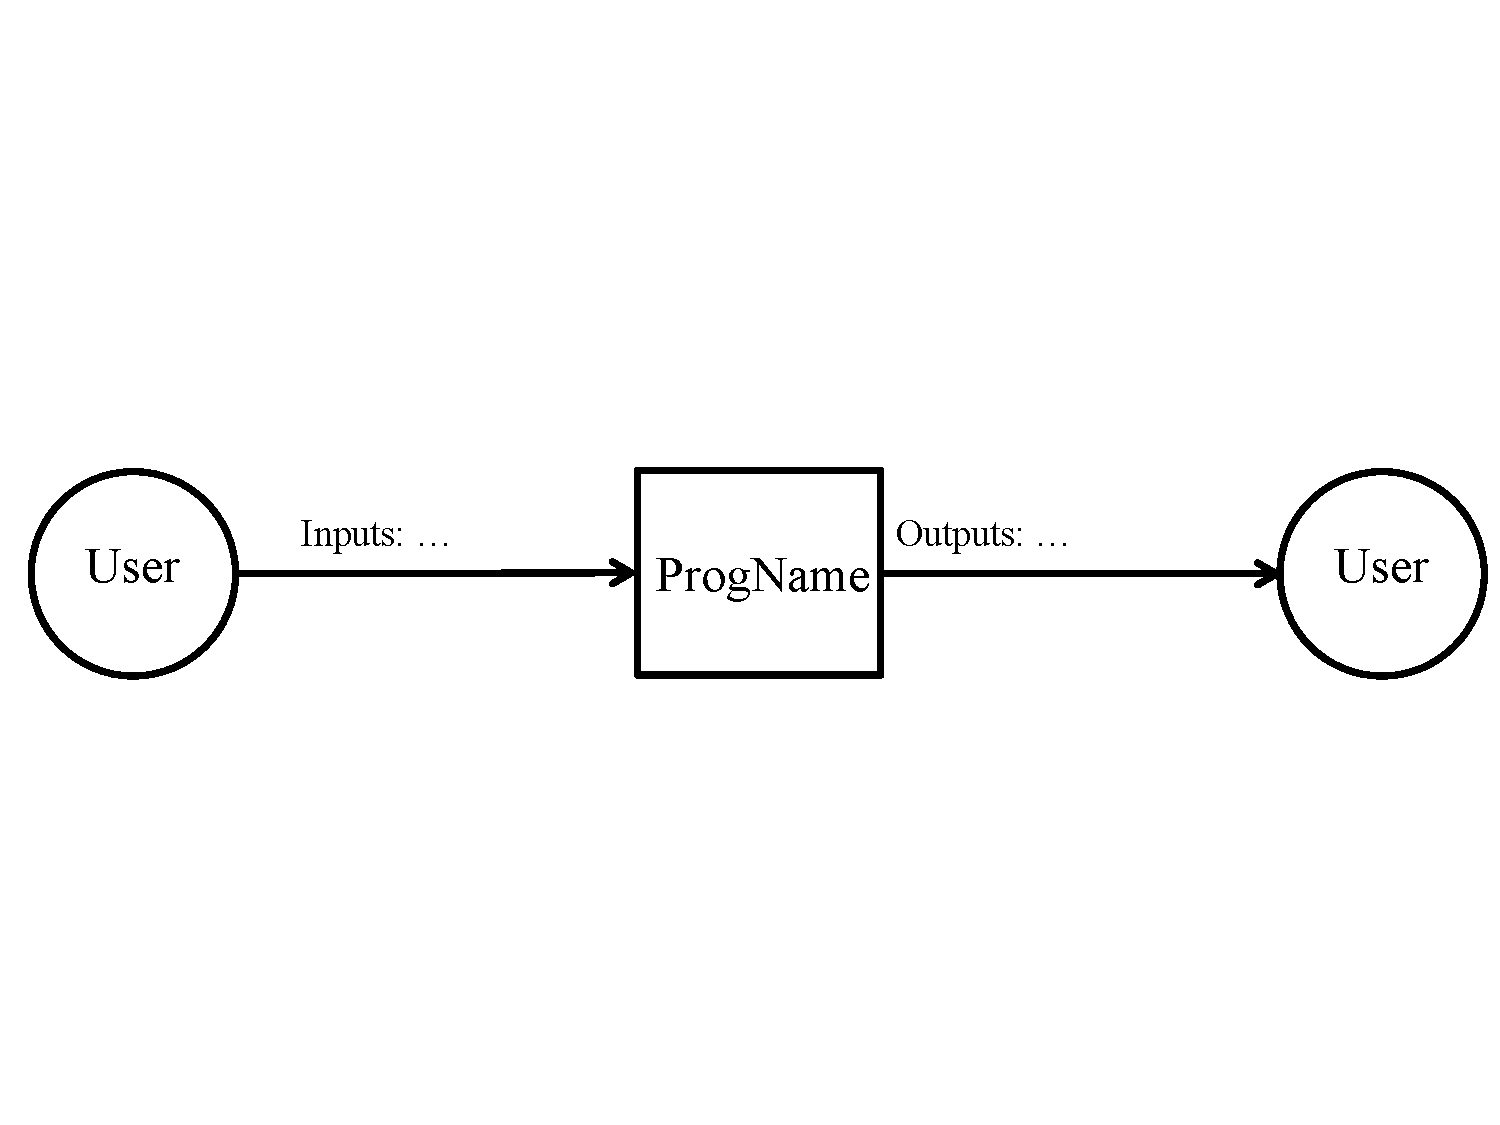
\includegraphics[width=0.6\textwidth]{figures/SystemContextFigure}
\caption{System Context}
\label{Fig_SystemContext} 
\end{center}
\end{figure}

\plt{For each of the entities in the system context diagram its responsibilities
  should be listed.  Whenever possible the system should check for data quality,
  but for some cases the user will need to assume that responsibility.  The list
  of responsibilities should be about the inputs and outputs only, and they
  should be abstract.  Details should not be presented here.  However, the
  information should not be so abstract as to just say ``inputs'' and
  ``outputs''.  A summarizing phrase can be used to characterize the inputs.
  For instance, saying ``material properties'' provides some information, but it
  stays away from the detail of listing every required properties.}

\begin{itemize}
\item User Responsibilities:
\begin{itemize}
\item 
\end{itemize}
\item \progname{} Responsibilities:
\begin{itemize}
\item Detect data type mismatch, such as a string of characters instead of a
  floating point number
\item 
\end{itemize}
\end{itemize}

\plt{Identify in what context the software will typically be used.  Is it for
exploration? education? engineering work? scientific work?. Identify whether it
will be used for mission-critical or safety-critical applications.} \plt{This
additional context information is needed to determine how much effort should be
devoted to the rationale section.  If the application is safety-critical, the
bar is higher.  This is currently less structured, but analogous to, the idea to
the Automotive Safety Integrity Levels (ASILs) that McSCert uses in their
automotive hazard analyses.}

\wss{The }
\subsection{User Characteristics} \label{SecUserCharacteristics}

\plt{This section summarizes the knowledge/skills expected of the user.
  Measuring usability, which is often a required non-function requirement,
  requires knowledge of a typical user.  As mentioned above, the user is a
  different role from the ``intended reader,'' as given in
  Section~\ref{sec_IntendedReader}.  As in Section~\ref{sec_IntendedReader}, the
  user characteristics should be specific an unambiguous.  For instance, ``The
  end user of \progname{} should have an understanding of undergraduate Level 1
  Calculus and Physics.''}

  This section summarizes the knowledge and skills expected of the user:
  
  \begin{itemize}
      \item The end user of the Yahtzee 3D game should have an understanding of the Yahtzee game, including its rules and strategies.
      
      \item Users should have a undergraduate level of understanding of probability theory, as it is important for comprehending the game's mechanics and making informed decisions during gameplay.
      
      \item A foundational knowledge of 3D environments and interactions may enhance the user's experience but is not strictly required.
  \end{itemize}
  

\subsection{System Constraints}

\plt{System constraints differ from other type of requirements because they
  limit the developers' options in the system design and they identify how the
  eventual system must fit into the world. This is the only place in the SRS
  where design decisions can be specified.  That is, the quality requirement for
  abstraction is relaxed here.  However, system constraints should only be
  included if they are truly required.}